%   DOCUMENT CLASS  %%%%%%%%%%%%%%%%%%%%%%%%%%%%%%%%%%%%%%%%%%%%%%%%%%%%%%%%%%%
%
%   Use the `sfuthesis` class to format your thesis. If your program does not
%   require a thesis defence, use the class option `undefended` like so:
%
%     \documentclass[undefended]{sfuthesis}
%
%   To generate a signature page for your defence, use the `sfuapproval` class
%   instead, by replacing the below line with
%
%     \documentclass{sfuapproval}
%
%   For more information about thesis formatting requirements, go to
%
%     http://www.lib.sfu.ca/help/publish/thesis
%
%   or ask a thesis advisor at the SFU Research Commons.
%
\documentclass{sfuthesis}
%   PACKAGES %%%%%%%%%%%%%%%%%%%%%%%%%%%%%%%%%%%%%%%%%%%%%%%%%%%%%%%%%%%%%%%%%%
%
%   Add any packages you need for your thesis here.
%   You don't need to call the following packages, which are already called in
%   the sfuthesis class file:
%
%   - appendix
%   - etoolbox
%   - fontenc
%   - geometry
%   - lmodern
%   - nowidow
%   - setspace
%   - tocloft
%
%   If you call one of the above packages (or one of their dependencies) with
%   options, you may get a "Option clash" LaTeX error. If you get this error,
%   you can fix it by removing your copy of \usepackage and passing the options
%   you need by adding
%
%       \PassOptionsToPackage{<options>}{<package>}
%
%   before \documentclass{sfuthesis}.
%
%   The following packages are a few suggestions you might find useful.
%
%   (1) amsmath and amssymb are essential if you have math in your thesis;
%       they provide useful commands like ``blackboard bold'' symbols and
%       environments for aligning equations.
%   (2) amsthm includes allows you to easily change the style and numbering of
%       theorems. It also provides an environment for proofs.
%   (3) graphicx allows you to add images with \includegraphics{filename}.
%   (4) hyperref turns your citations and cross-references into clickable
%       links, and adds metadata to the compiled PDF.
%   (5) pdfpages lets you import pages of external PDFs using the command
%       \includepdf{filename}. You will need to do this if your research
%       requires an Ethics Statement.
%

\usepackage{amsmath}                            % (1)
\usepackage{amssymb}                            % (1)
\usepackage{amsthm}                             % (2)
\usepackage{graphicx}                           % (3)
\usepackage[pdfborder={0 0 0}]{hyperref}        % (4)
% \usepackage{pdfpages}                         % (5)
% ...
% ...
% ...
% ... add your own packages here!
\usepackage[cache=false]{minted}
\usepackage{hyperref}
\usepackage{booktabs}
\usepackage{graphics}
\usepackage{xcolor}
\usepackage{bm}




%   OTHER CUSTOMIZATIONS %%%%%%%%%%%%%%%%%%%%%%%%%%%%%%%%%%%%%%%%%%%%%%%%%%%%%%
%
%   Add any packages you need for your thesis here. We've started you off with
%   a few suggestions.
%
%   (1) Use a single word space between sentences. If you disable this, you
%       will have to manually control spacing around abbreviations.
%   (2) Correct the capitalization of "Chapter" and "Section" if you use the
%       \autoref macro from the `hyperref` package.
%   (3) The LaTeX thesis template defaults to one-and-a-half line spacing. If
%       your supervisor prefers double-spacing, you can redefine the
%       \defaultspacing command.
%

\frenchspacing                                    % (1)
\renewcommand*{\chapterautorefname}{Chapter}      % (2)
\renewcommand*{\sectionautorefname}{Section}      % (2)
\renewcommand*{\subsectionautorefname}{Section}   % (2)
% \renewcommand{\defaultspacing}{\doublespacing}  % (3)
% ...
% ...
% ...
% ... add your own customizations here!


\graphicspath{{img/}}



\begin{document}
%   FRONTMATTER  %%%%%%%%%%%%%%%%%%%%%%%%%%%%%%%%%%%%%%%%%%%%%%%%%%%%%%%%%%%%%%
%
%   Title page, committee page, copyright declaration, abstract,
%   dedication, acknowledgements, table of contents, etc.
%
%   If your research requires an Ethics Statement, download one from the
%   SFU library website and uncomment the appropriate lines below.
%

%   DOCUMENT METADATA  %%%%%%%%%%%%%%%%%%%%%%%%%%%%%%%%%%%%%%%%%%%%%%%%%%%%%%%%
%
%   Fill in the following information for the title page and approval page.
%

\title{An Analysis of Missing Transverse Momentum Triggers for Improving Efficiency at the ATLAS Experiment at CERN}
\thesistype{Thesis}
\author{Joseph Corrado}
\degree{Bachelors with Honors}
\previousdegrees{}
\discipline{Physics}
\department{Department of Physics}
\faculty{Faculty of NYU Physics}
\copyrightyear{2019}
\semester{Spring 2019}
\date{May 20th, 2019}

\keywords{}
\committee{%
	\chair{Allen Mincer}{Senior Supervisor\\Professor}
	\member{Kyle Cranmer}{Professor}
	\member{Daniel Zwanziger}{Dean of Undergraduate Studies\\Professor}
}

%   PACKAGES %%%%%%%%%%%%%%%%%%%%%%%%%%%%%%%%%%%%%%%%%%%%%%%%%%%%%%%%%%%%%%%%%%
%
%   Add any packages you need for your thesis here.
%   You don't need to call the following packages, which are already called in
%   the sfuthesis class file:
%
%   - appendix
%   - etoolbox
%   - fontenc
%   - geometry
%   - lmodern
%   - nowidow
%   - setspace
%   - tocloft
%
%   If you call one of the above packages (or one of their dependencies) with
%   options, you may get a "Option clash" LaTeX error. If you get this error,
%   you can fix it by removing your copy of \usepackage and passing the options
%   you need by adding
%
%       \PassOptionsToPackage{<options>}{<package>}
%
%   before \documentclass{sfuthesis}.
%
%   The following packages are a few suggestions you might find useful.
%
%   (1) amsmath and amssymb are essential if you have math in your thesis;
%       they provide useful commands like ``blackboard bold'' symbols and
%       environments for aligning equations.
%   (2) amsthm includes allows you to easily change the style and numbering of
%       theorems. It also provides an environment for proofs.
%   (3) graphicx allows you to add images with \includegraphics{filename}.
%   (4) hyperref turns your citations and cross-references into clickable
%       links, and adds metadata to the compiled PDF.
%   (5) pdfpages lets you import pages of external PDFs using the command
%       \includepdf{filename}. You will need to do this if your research
%       requires an Ethics Statement.
%


%   OTHER CUSTOMIZATIONS %%%%%%%%%%%%%%%%%%%%%%%%%%%%%%%%%%%%%%%%%%%%%%%%%%%%%%
%
%   Add any packages you need for your thesis here. We've started you off with
%   a few suggestions.
%
%   (1) Use a single word space between sentences. If you disable this, you
%       will have to manually control spacing around abbreviations.
%   (2) Correct the capitalization of "Chapter" and "Section" if you use the
%       \autoref macro from the `hyperref` package.
%   (3) The LaTeX thesis template defaults to one-and-a-half line spacing. If
%       your supervisor prefers double-spacing, you can redefine the
%       \defaultspacing command.
%

\frenchspacing                                    % (1)
\renewcommand*{\chapterautorefname}{Chapter}      % (2)
\renewcommand*{\sectionautorefname}{Section}      % (2)
\renewcommand*{\subsectionautorefname}{Section}   % (2)
% \renewcommand{\defaultspacing}{\doublespacing}  % (3)
% ...
% ...
% ...
% ... add your own customizations here!




%   FRONTMATTER  %%%%%%%%%%%%%%%%%%%%%%%%%%%%%%%%%%%%%%%%%%%%%%%%%%%%%%%%%%%%%%
%
%   Title page, committee page, copyright declaration, abstract,
%   dedication, acknowledgements, table of contents, etc.
%
%   If your research requires an Ethics Statement, download one from the
%   SFU library website and uncomment the appropriate lines below.
%


\frontmatter
\maketitle{}
\makecommittee{}

%\addtoToC{Ethics Statement}%
%\includepdf[pagecommand={\thispagestyle{plain}}]{ethicsstatement.pdf}%
%\clearpage

\begin{abstract}
	This is a blank document from which you can start writing your thesis.
\end{abstract}

\begin{dedication}
	This is an optional page.
\end{dedication}

\begin{acknowledgements}
	This is an optional page.
\end{acknowledgements}


\addtoToC{Table of Contents}%
\tableofcontents%
\clearpage

\addtoToC{List of Tables}%
\listoftables%
\clearpage

\addtoToC{List of Figures}%
\listoffigures%
\clearpage


%   MAIN MATTER  %%%%%%%%%%%%%%%%%%%%%%%%%%%%%%%%%%%%%%%%%%%%%%%%%%%%%%%%%%%%%%
%
%   Start writing your thesis --- or start \include ing chapters --- here.
%

\mainmatter%

\chapter{Introduction}

By default, only works cited in the text will be added to the bibliography~\cite{latexcompanion}.

\chapter{Improving Efficiency Using Combined Algorithms}
For our project, we wanted to improve the efficiency of the algorithms in classifying the MET of a signal event as larger than some MET. The way we do this is by determining the thresholds needed to satisfy the trigger rate based on the fraction of background events kept by the trigger system, and then by using those thresholds to compute an efficiency for the same pair of algorithms to classify a signal event as larger than some value of MET.
By signal events, we mean events for which the muon trigger fired, which correspond to events for which a muon was detected.
In this assignment, we wanted to see if we could obtain an increase in efficiency by combining uncorrelated algorithms together subject to the constraint of the trigger rate. The issue is that there are many pairs of thresholds that when combine will keep the proper trigger rate. In the parameter space of all possible combinations of combined thresholds, we have two degrees of freedom in determining what the appropriate thresholds on a pair of algorithms should be. 
In order to simplify the problem, I imposed the constraint that the two trigger rates for the algorithms had to be the same. Therefore, I removed a degree of freedom in the parameter space by constraining my solution space to pairs of thresholds that satisfy the trigger rate and lie on the line $y=x$. The monotonicity of the fraction of events kept as you change either of the thresholds on the algorithms guarantees that there will be a unique solution to both of these constraints on the parameter space. \\
Once we added the constraint of keeping the same fraction individually, the problem essentially became one-dimensional, and I used the popular bisection root-finding method in order to compute the solution to the optimal pair of thresholds. \\
This consisted of guessing an individual fraction for each of the algorithms to keep, and then computing what the combined fraction of events kept was. We iterated this process until the combined fraction kept matched the trigger rate to within one bin.
The level curve describing the set of pairs of thresholds such that the trigger rate constraint is satisfied is given by the constraint:
$$f(\tau_{\alpha},\tau_{\beta})=C$$
for some $C$. Here, $f$ is the function representing the fraction of events kept when the algorithms are used together at the same time. 
This $C$ is determined by the fraction of background events that are kept by the trigger system. 
In order to compute $C$, we used the fraction of passnoalg data that passed an L1 MET cut of $50$ GeV and a CELL MET cut of $100$ GeV. 
For our analysis, $C$ turned out to be $0.0059$.
So we needed to solve the equation $f(\tau_{\alpha},\tau_{\beta})=0.0059$. 
However, because the parameter space is two-dimensional, and the evaluation of $f$ takes a long time (fraction of events kept by both algorithms, and by each one individually), we introduced the constraint that the two individual fractions kept needed to be the same.
In summary, we use the background events in order to compute what the thresholds on the algorithms need to be in order to keep the trigger rate, and then we determine the efficiencies of this combination of algorithms at those thresholds from the signal events. 
\section{Signal Selection on Transverse Mass}
In addition to the cuts on the various algorithms, we also needed to introduce a cut on the transverse mass that is detected to ensure we only keep events with a transverse mass close to that of the W boson ($80.379\pm 0.012 GeV/c^2$). 
We compute the transverse mass using:
$$m_{T}=\sqrt{2P_{\mu}P_{\nu}(1+\cos{(\phi)})}$$
In addition to the previously mentioned cuts, we also added a cut on the transverse mass for the range $40 \leq m_{T} \leq 100$. 
This was necessary in order to select signal events that are likely to have a high rate of weakly interacting particles produced.
\pagebreak
\section{Results}
\subsection{Algorithms that did not do better combined}
For most pairs of algorithms, we found that combining algorithms such that they keep the correct trigger rate did not yield any gain in efficiency. As in figure \ref{no_gain_efficiency}, we see that the red curve lies underneath the green curve. 
\begin{figure}[h]
        \centering
        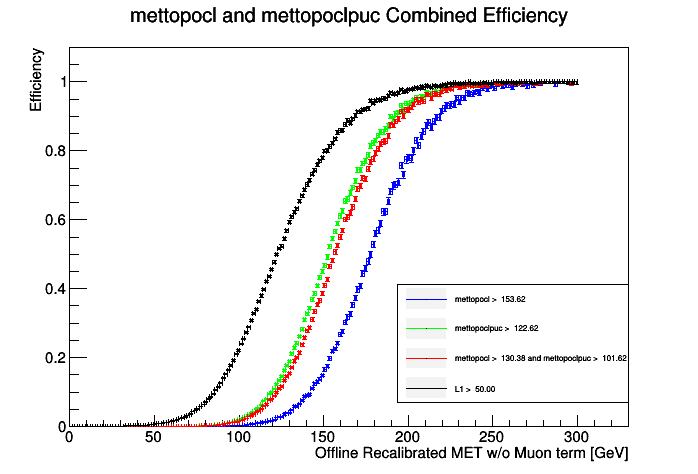
\includegraphics[scale=0.4]{topocl_puc_efficiencies}
        \caption{Efficiencies of METTOPOCL and METTOPOCLPUC}
        \label{no_gain_efficiency}
\end{figure}
\clearpage
\subsection{Algorithms that did do better combined}
We found that we were able to achieve an increase in the overall efficiency for some of the pairs of algorithms considered. 
\begin{figure}[h]
        \centering
        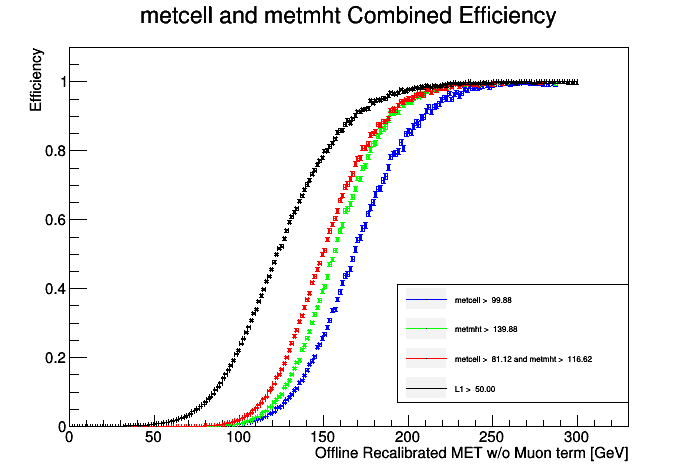
\includegraphics[scale=0.4]{cell_mht_efficiencies}
        \caption{Efficiencies of METCELL and METMHT}
\end{figure}
\begin{figure}[h]
        \centering
        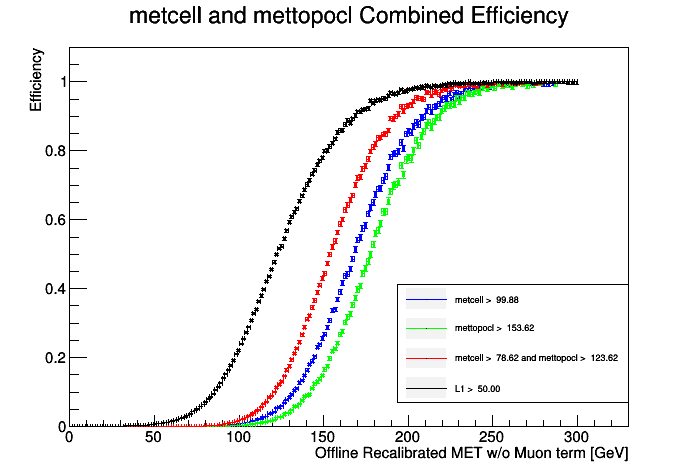
\includegraphics[scale=0.4]{cell_topocl_efficiencies}
        \caption{Efficiencies of METCELL and METTOPOCL}
\end{figure}
\begin{figure}[h]
        \centering
        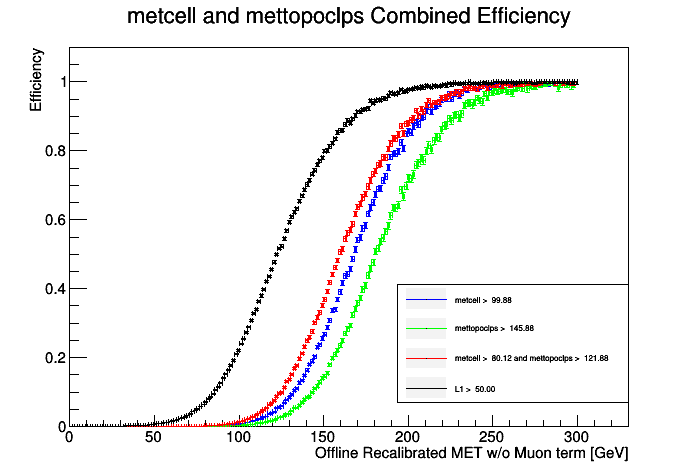
\includegraphics[scale=0.4]{cell_ps_efficiencies}
        \caption{Efficiencies of METCELL and METMHT}
\end{figure}
\begin{figure}[h]
        \centering
        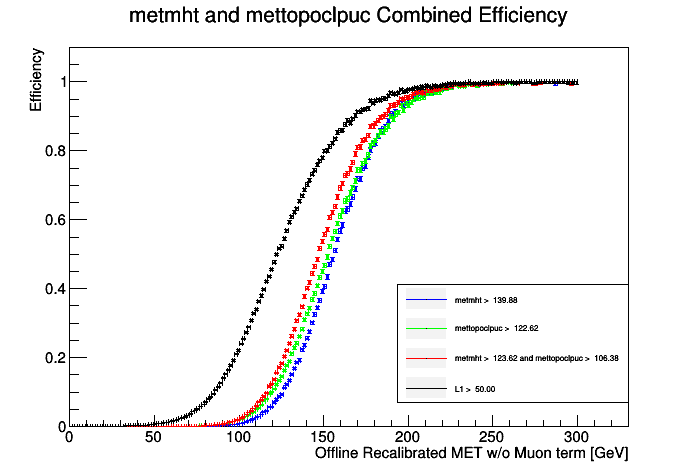
\includegraphics[scale=0.4]{mht_puc_efficiencies}
        \caption{Efficiencies of METCELL and METTOPOCL}
\end{figure}
\clearpage
\subsection{Best Combined Algorithms and Best Individual Algorithms}
During the summer of 2018, the pufit plus cell algorithm trigger was the main one that was actually used for the second part of Run 2.
In figure \ref{bisection_fig}, I've plotted the efficiencies of the best combined algorithms along with the best efficiencies of the individual algorithms. We see that the top curves on this plot are those for combined algorithms, as well as the individual mettopoclpuc and metmht curves.
\begin{figure}[h]
        \centering
        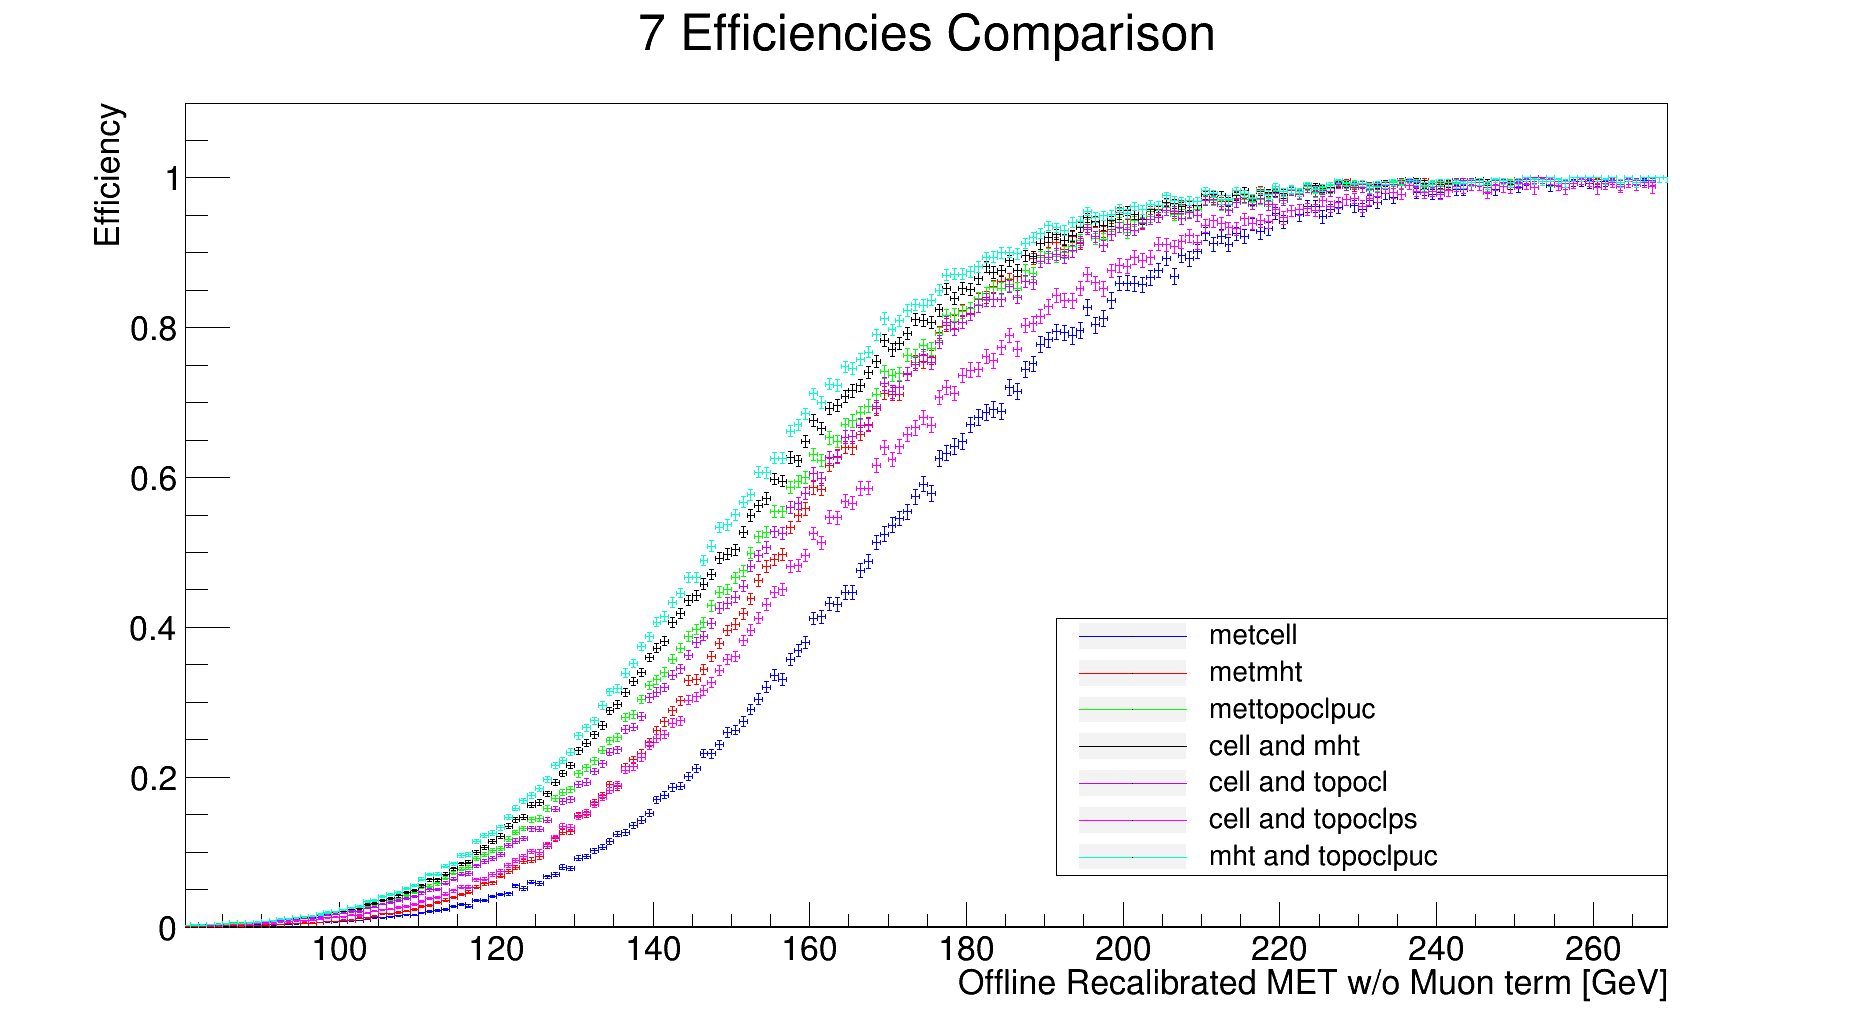
\includegraphics[scale=0.2]{7Efficiencies}
        \caption{Best Combined Efficiency Algorithms Versus Best Individual Algorithms}
        \label{bisection_fig}
\end{figure}
\clearpage

\section{Predicting the unbiased MET Distribution at Higher Luminosity}
Our goal is to empirically reconstruct the unbiased MET distribution using ZeroBias HLT noalg L1XE30 and HLT noalg L1XE50 data. 
We want to use this data to determine the CELL MET distribution as a function of $\mu$.
Because the zerobias events only allow us to go up to about $80$ GeV, we use the \texttt{HLTnoalg\_L1XExx} triggered events in order to extend to higher MET.
We correct the \texttt{HLTnoalg\_L1XExx} data using the efficiency curves determined from lower threshold triggers.
In addition to performing this correction, we needed to propagate the errors properly on the corrected distribution because it depends on the fit functions to the efficiency in which the fitting parameters have some uncertainty. 
In order to do the reconstruction, we needed to perform several steps:
\begin{enumerate}
        \item compute the efficiency of $L1>30$GeV for \texttt{HLT\_ZB\_L1ZB} data as a function of CELL MET
        \item correct the \texttt{HLT\_ZB\_L1XE30} data back to the \texttt{HLT\_ZB\_L1ZB} distribution by multiplying by the prescale and dividing by the efficiency. 
        \item compute the efficiency of $L1>50GeV$ for \texttt{HLT\_ZB\_L1XE30} data as a function of CELL MET
        \item correct the \texttt{HLT\_ZB\_L1XE50} data back to the \texttt{HLT\_ZB\_L1ZB} distribution by multiplying by the corresponding prescale, and dividing by both of the previously computed efficiencies. 
\end{enumerate}
For this project, we used the 2015, 2016 and 2017 combined \texttt{HLTnoalg\_L1Z} , \texttt{HLTnoalg\_L1XE30} and \texttt{HLTnoalg\_L1XE50} data produced by Jonathan Burr on 11/17/2017 from the zerobias and JETM10 trees.
In addition, we removed the events from runs 330203, 331975 and 334487 because these events had large MET events without jets and the logbook says there were calorimeter noise problems in these runs. 


%   BACK MATTER  %%%%%%%%%%%%%%%%%%%%%%%%%%%%%%%%%%%%%%%%%%%%%%%%%%%%%%%%%%%%%%
%
%   References and appendices. Appendices come after the bibliography and
%   should be in the order that they are referred to in the text.
%
%   If you include figures, etc. in an appendix, be sure to use
%
%       \caption[]{...}
%
%   to make sure they are not listed in the List of Figures.
%

\backmatter%
	\addtoToC{Bibliography}
	\bibliographystyle{plain}
	\bibliography{references}

\begin{appendices} % optional
	\chapter{Code}
\end{appendices}
\end{document}
